\chapter{Conclusioni}

\section{Sintesi del Lavoro}
Questa tesi ha ripercorso l'evoluzione degli strumenti 
computazionali applicati alla pipeline di sviluppo farmaceutico, 
con un focus sulla predizione delle interazioni farmaco-bersaglio 
e sulla valutazione delle proprietà ADMET. 
Il filo conduttore 
che attraversa tutti i capitoli è il modo in cui la ricerca si è trasformata da un 
processo empirico incerto a un 
problema computazionale di ottimizzazione in spazi ad alta dimensionalità, 
affrontabile attraverso strumenti di apprendimento automatico.

Il capitolo sulla rappresentazione molecolare ha mostrato come 
il primo ostacolo computazionale, ovvero la traduzione di entità biochimiche 
complesse in formati leggibili ed elaborabili da algoritmi, sia stato 
affrontato attraverso rappresentazioni progressivamente più 
espressive:

dalle stringhe SMILES ai fingerprint molecolari, 
fino ai grafi molecolari che preservano la topologia e le caratteristiche
stereochimiche particolari alle singole molecole. 

Il capitolo sulla DTI e DTA ha mostrato come la formalizzazione 
del problema computazionale abbia 
permesso di riformulare la ricerca farmacologica in due task 
distinti di apprendimento supervisionato:

\textbf{classificazione binaria} per la presenza dell'interazione e \textbf{regressione} su valore continuo per 
la stima quantitativa dell'affinità. L'evoluzione dei metodi, 
dai modelli lineari QSAR al docking molecolare fino alle 
architetture di Deep Learning, rispecchia l'avanzamento tecnologico moderno e la crescente
complessità delle relazioni che i modelli sono chiamati a 
catturare.

Il capitolo ADMET ha completato il quadro mostrando come la 
valutazione della sicurezza farmacologica, storicamente 
relegata alle fasi cliniche avanzate, possa essere anticipata 
computazionalmente, riducendo il tasso di logoramento dei 
candidati nelle fasi più costose della pipeline.
\section{Lo Stato dell'Arte e le Sfide Aperte}
Nonostante i progressi documentati, il campo presenta sfide 
algoritmiche e metodologiche ancora aperte che condizionano 
l'affidabilità e la generalizzabilità dei modelli.

Il \textbf{cold-start problem} rimane la sfida critica più 
rilevante. Sebbene molti algoritmi eccellano in scenari "warm", in cui le molecole del Test-Set assomigliano a quelle dell'addestramento, la predizione di interazioni per farmaci o target \textbf{mai 
osservati} durante il \textit{training} richiede modelli con 
capacità di generalizzazione induttiva che le architetture 
attuali possiedono solo parzialmente \cite{wangUnifiedSurveyDrugtarget2026a}.
\begin{figure}
    \centering
    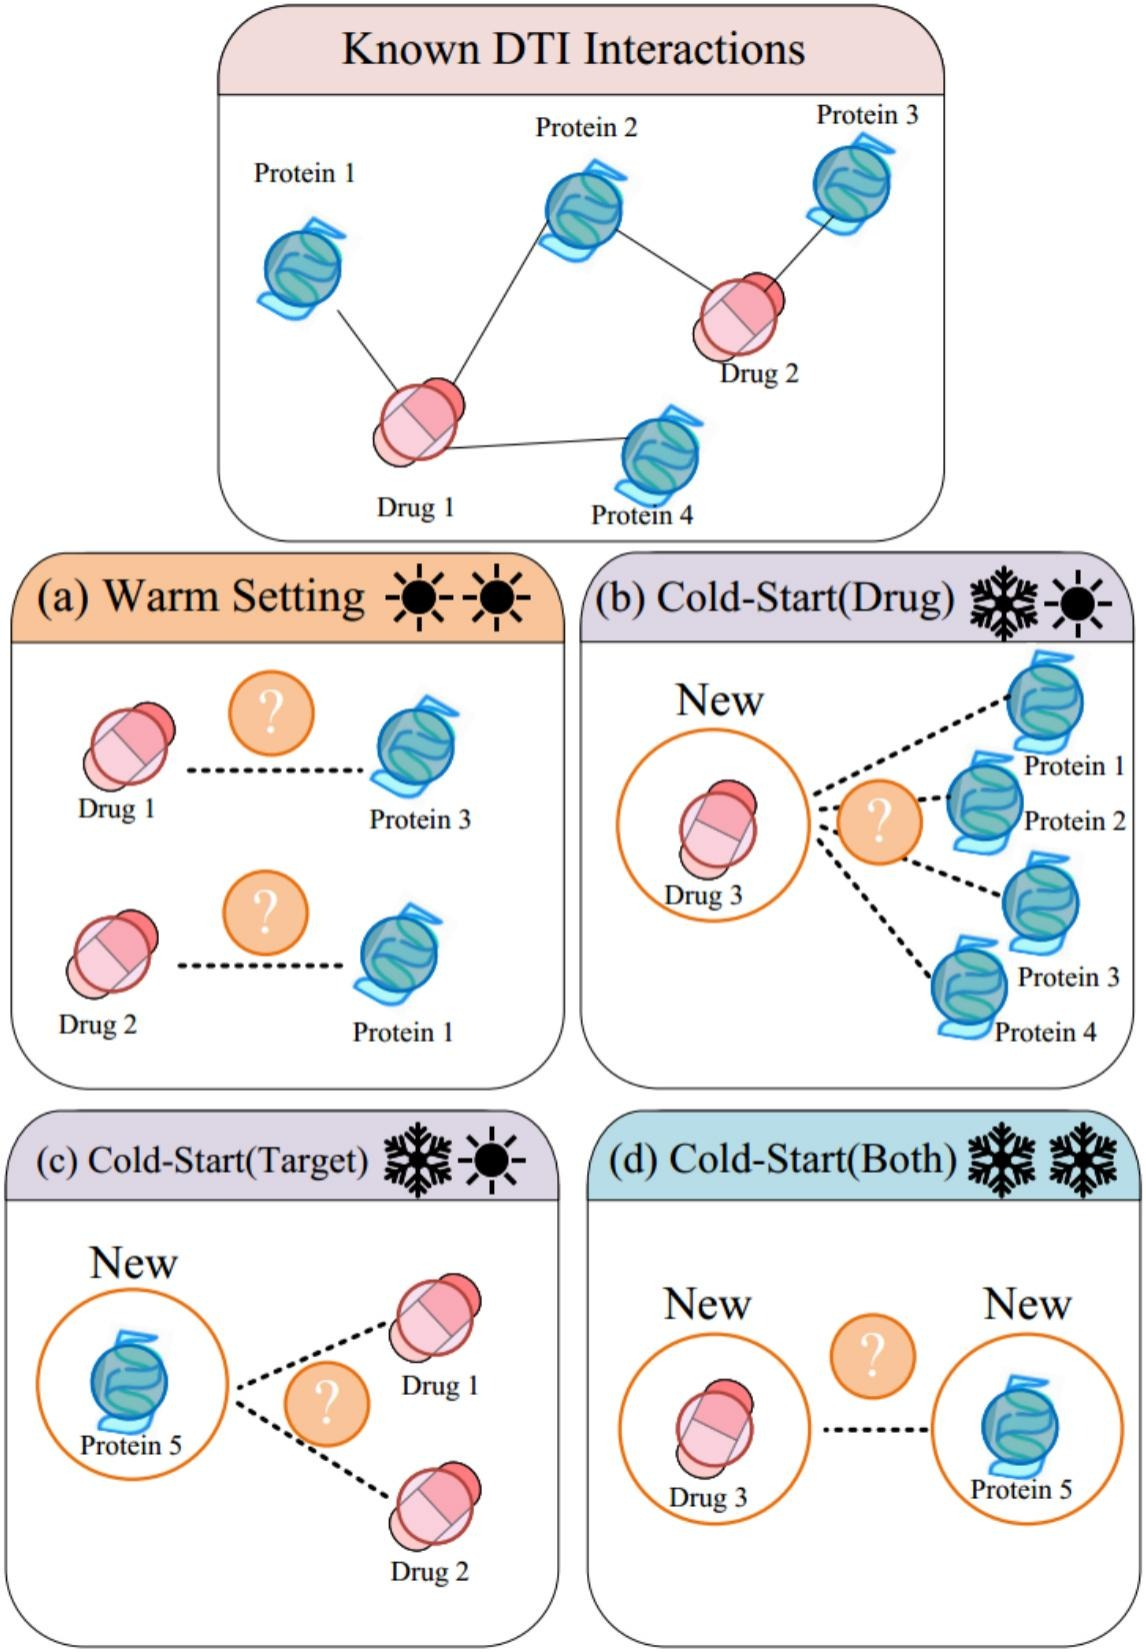
\includegraphics[width=0.5\linewidth]{figures/cold_start.png}
    \caption{(a) Warm-Start: il modello prevede interazioni tra farmaci e target già presenti nel training set. (b) Cold-Start (Drug): predizione per un nuovo farmaco mai visto prima. (c) Cold-Start (Target): predizione per una nuova proteina bersaglio. (d) Cold-Start (Both): scenario di massima complessità in cui sia il farmaco che il target sono inediti.
    Figura riprodotta con il permesso di Elsevier, da Wang et al., A unified survey on drug-target interaction and binding affinity prediction: Models, representations, and challenges", Biotechnology Advances, 2026. Licenza numero: 6286991125834.}
    \label{fig:placeholder}
\end{figure}
I modelli basati su 
Transformer e i PLM mostrano la maggiore robustezza in 
questi scenari, grazie alla conoscenza biochimica generale 
acquisita durante il pre-training, che permette loro di colmare l'assenza di esempi specifici.
Tuttavia, la questione rimane ancora
aperta per target biologicamente distanti da quelli 
rappresentati nei dataset, che rappresentano vere e proprie "zone inesplorate" dello spazio chimico.

Lo \textbf{sbilanciamento dei dati} costituisce un problema 
strutturale della classificazione per cui i dataset DTI contengono molte più coppie 
non interagenti che interagenti, e in cui molte coppie etichettate 
come negative sono in realtà non testate.

Questo sbilanciamento porta i modelli a essere eccessivamente ottimisti nelle predizioni (che sono portate a seguire la classe maggioritaria) e a fallire nell'identificazione di interazioni rare ma biologicamente significative.

Tecniche come 
SMOTE (\textit{Synthetic Minority Over-sampling Technique}) e sampling randomico \cite{ahmadMachineLearningDrugtarget2026} mitigano parzialmente il problema e aiutano a ridurre l'\textit{overfitting}, 
ma non lo risolvono alla radice, che risiede nella natura 
stessa dei dati sperimentali disponibili. Infatti, visto che i dataset forniti includono spesso solo interazioni note, trattando tutte le altre coppie come negative, le metriche di validazione della classificazione, ad esempio AUROC (\textit{Area Under the Receiver Operating Characteristic curve}), possono risultare "gonfiate" artificialmente, portando a scarse prestazioni \cite{ahmadMachineLearningDrugtarget2026}.

Infine, come menzionato in precedenza, l'\textbf{interpretabilità} dei modelli deep learning 
rappresenta un requisito necessario per l'approvazione e 
l'adozione clinica \cite{wangUnifiedSurveyDrugtarget2026a}. 
Le mappe di \textit{Attention}, soprattutto nel contesto di predizione ADMET, hanno aperto la strada alla validazione biologica 
delle predizioni, ma rimangono processi non investigabili e difficili da seguire nella loro esecuzione "Black Box".

La mancanza di spiegazioni trasparenti ostacola l'accettazione dei medicinali individuati da parte delle aziende regolatorie.
\section{Riflessioni Finali}
I metodi 
computazionali studiati non hanno sostituito la validazione 
sperimentale, ma l'hanno resa più mirata, riducendo 
drasticamente lo spazio di ricerca da esplorare in 
laboratorio, concentrando le risorse sui candidati più promettenti.

I casi di studio descritti suggeriscono che i progressi 
futuri più significativi non deriveranno 
dall'affinamento di singole architetture, ma dalla capacità di scegliere la combinazione più appropriata
di rappresentazione e modello in funzione della natura del problema:

In particolare le architetture di tipo \textbf{ibrido} (come TC-DTA) si dimostrano ideali per fornire un buon compromesso tra l'efficienza di predizione e l'accuratezza della rappresentazione. Separando l'elaborazione del farmaco e del target in due rami paralleli, il modello ottimizza l'analisi delle feature su scale diverse.

Inoltre, la crescente 
disponibilità di dati biologici annotati, unita 
allo sviluppo di PLM specializzati per il dominio 
chimico e proteico, suggerisce che il gap tra 
predizione computazionale e validazione clinica 
sia destinato a ridursi ulteriormente nei prossimi 
anni.

\begin{table}[h]
\centering
\renewcommand{\arraystretch}{1.3}
\begin{tabularx}{\textwidth}{|p{2.3cm}|X|X|}
\hline
\textbf{Modello} & \textbf{Punti di forza} & \textbf{Limiti} \\
\hline
CNN &
Scalabilità, efficienza computazionale, buona estrazione di motif locali &
Difficoltà a catturare dipendenze a lungo raggio e contesto 3D \\
\hline
RNN &
Memoria contestuale, adatta a stringhe di lunghezza variabile &
Inefficiente su sequenze lunghe. Nessuna nozione di topologia spaziale \\
\hline
GNN &
Rappresentazione molto fedele alla topologia chimica &
Costo computazionale del message passing alto \\
\hline
Transformer / PLM &
Cattura dipendenze a lungo raggio. Interpretabile tramite mappe di attenzione. Robustezza in scenari Cold-Start &
Complessità e costi elevati in fase di training \\
\hline
TC-DTA (ibrido) &
Combina l'efficienza della CNN sul farmaco con la modellazione di dipendenze globali sulla proteina &
Architettura più complessa da addestrare rispetto ai singoli moduli \\
\hline
\end{tabularx}
\caption{Sintesi delle architetture di Deep Learning per la predizione DTI/DTA e relative caratteristiche emerse dalla letteratura analizzata.}
\label{tab:modelli_dti_dta}
\end{table}
